\documentclass[1p]{elsarticle_modified}
%\bibliographystyle{elsarticle-num}

%\usepackage[colorlinks]{hyperref}
%\usepackage{abbrmath_seonhwa} %\Abb, \Ascr, \Acal ,\Abf, \Afrak
\usepackage{amsfonts}
\usepackage{amssymb}
\usepackage{amsmath}
\usepackage{amsthm}
\usepackage{scalefnt}
\usepackage{amsbsy}
\usepackage{kotex}
\usepackage{caption}
\usepackage{subfig}
\usepackage{color}
\usepackage{graphicx}
\usepackage{xcolor} %% white, black, red, green, blue, cyan, magenta, yellow
\usepackage{float}
\usepackage{setspace}
\usepackage{hyperref}

\usepackage{tikz}
\usetikzlibrary{arrows}

\usepackage{multirow}
\usepackage{array} % fixed length table
\usepackage{hhline}

%%%%%%%%%%%%%%%%%%%%%
\makeatletter
\renewcommand*\env@matrix[1][\arraystretch]{%
	\edef\arraystretch{#1}%
	\hskip -\arraycolsep
	\let\@ifnextchar\new@ifnextchar
	\array{*\c@MaxMatrixCols c}}
\makeatother %https://tex.stackexchange.com/questions/14071/how-can-i-increase-the-line-spacing-in-a-matrix
%%%%%%%%%%%%%%%

\usepackage[normalem]{ulem}

\newcommand{\msout}[1]{\ifmmode\text{\sout{\ensuremath{#1}}}\else\sout{#1}\fi}
%SOURCE: \msout is \stkout macro in https://tex.stackexchange.com/questions/20609/strikeout-in-math-mode

\newcommand{\cancel}[1]{
	\ifmmode
	{\color{red}\msout{#1}}
	\else
	{\color{red}\sout{#1}}
	\fi
}

\newcommand{\add}[1]{
	{\color{blue}\uwave{#1}}
}

\newcommand{\replace}[2]{
	\ifmmode
	{\color{red}\msout{#1}}{\color{blue}\uwave{#2}}
	\else
	{\color{red}\sout{#1}}{\color{blue}\uwave{#2}}
	\fi
}

\newcommand{\Sol}{\mathcal{S}} %segment
\newcommand{\D}{D} %diagram
\newcommand{\A}{\mathcal{A}} %arc


%%%%%%%%%%%%%%%%%%%%%%%%%%%%%5 test

\def\sl{\operatorname{\textup{SL}}(2,\Cbb)}
\def\psl{\operatorname{\textup{PSL}}(2,\Cbb)}
\def\quan{\mkern 1mu \triangleright \mkern 1mu}

\theoremstyle{definition}
\newtheorem{thm}{Theorem}[section]
\newtheorem{prop}[thm]{Proposition}
\newtheorem{lem}[thm]{Lemma}
\newtheorem{ques}[thm]{Question}
\newtheorem{cor}[thm]{Corollary}
\newtheorem{defn}[thm]{Definition}
\newtheorem{exam}[thm]{Example}
\newtheorem{rmk}[thm]{Remark}
\newtheorem{alg}[thm]{Algorithm}

\newcommand{\I}{\sqrt{-1}}
\begin{document}

%\begin{frontmatter}
%
%\title{Boundary parabolic representations of knots up to 8 crossings}
%
%%% Group authors per affiliation:
%\author{Yunhi Cho} 
%\address{Department of Mathematics, University of Seoul, Seoul, Korea}
%\ead{yhcho@uos.ac.kr}
%
%
%\author{Seonhwa Kim} %\fnref{s_kim}}
%\address{Center for Geometry and Physics, Institute for Basic Science, Pohang, 37673, Korea}
%\ead{ryeona17@ibs.re.kr}
%
%\author{Hyuk Kim}
%\address{Department of Mathematical Sciences, Seoul National University, Seoul 08826, Korea}
%\ead{hyukkim@snu.ac.kr}
%
%\author{Seokbeom Yoon}
%\address{Department of Mathematical Sciences, Seoul National University, Seoul, 08826,  Korea}
%\ead{sbyoon15@snu.ac.kr}
%
%\begin{abstract}
%We find all boundary parabolic representation of knots up to 8 crossings.
%
%\end{abstract}
%\begin{keyword}
%    \MSC[2010] 57M25 
%\end{keyword}
%
%\end{frontmatter}

%\linenumbers
%\tableofcontents
%
\newcommand\colored[1]{\textcolor{white}{\rule[-0.35ex]{0.8em}{1.4ex}}\kern-0.8em\color{red} #1}%
%\newcommand\colored[1]{\textcolor{white}{ #1}\kern-2.17ex	\textcolor{white}{ #1}\kern-1.81ex	\textcolor{white}{ #1}\kern-2.15ex\color{red}#1	}

{\Large $\underline{11a_{120}~(K11a_{120})}$}

\setlength{\tabcolsep}{10pt}
\renewcommand{\arraystretch}{1.6}
\vspace{1cm}\begin{tabular}{m{100pt}>{\centering\arraybackslash}m{274pt}}
\multirow{5}{120pt}{
	\centering
	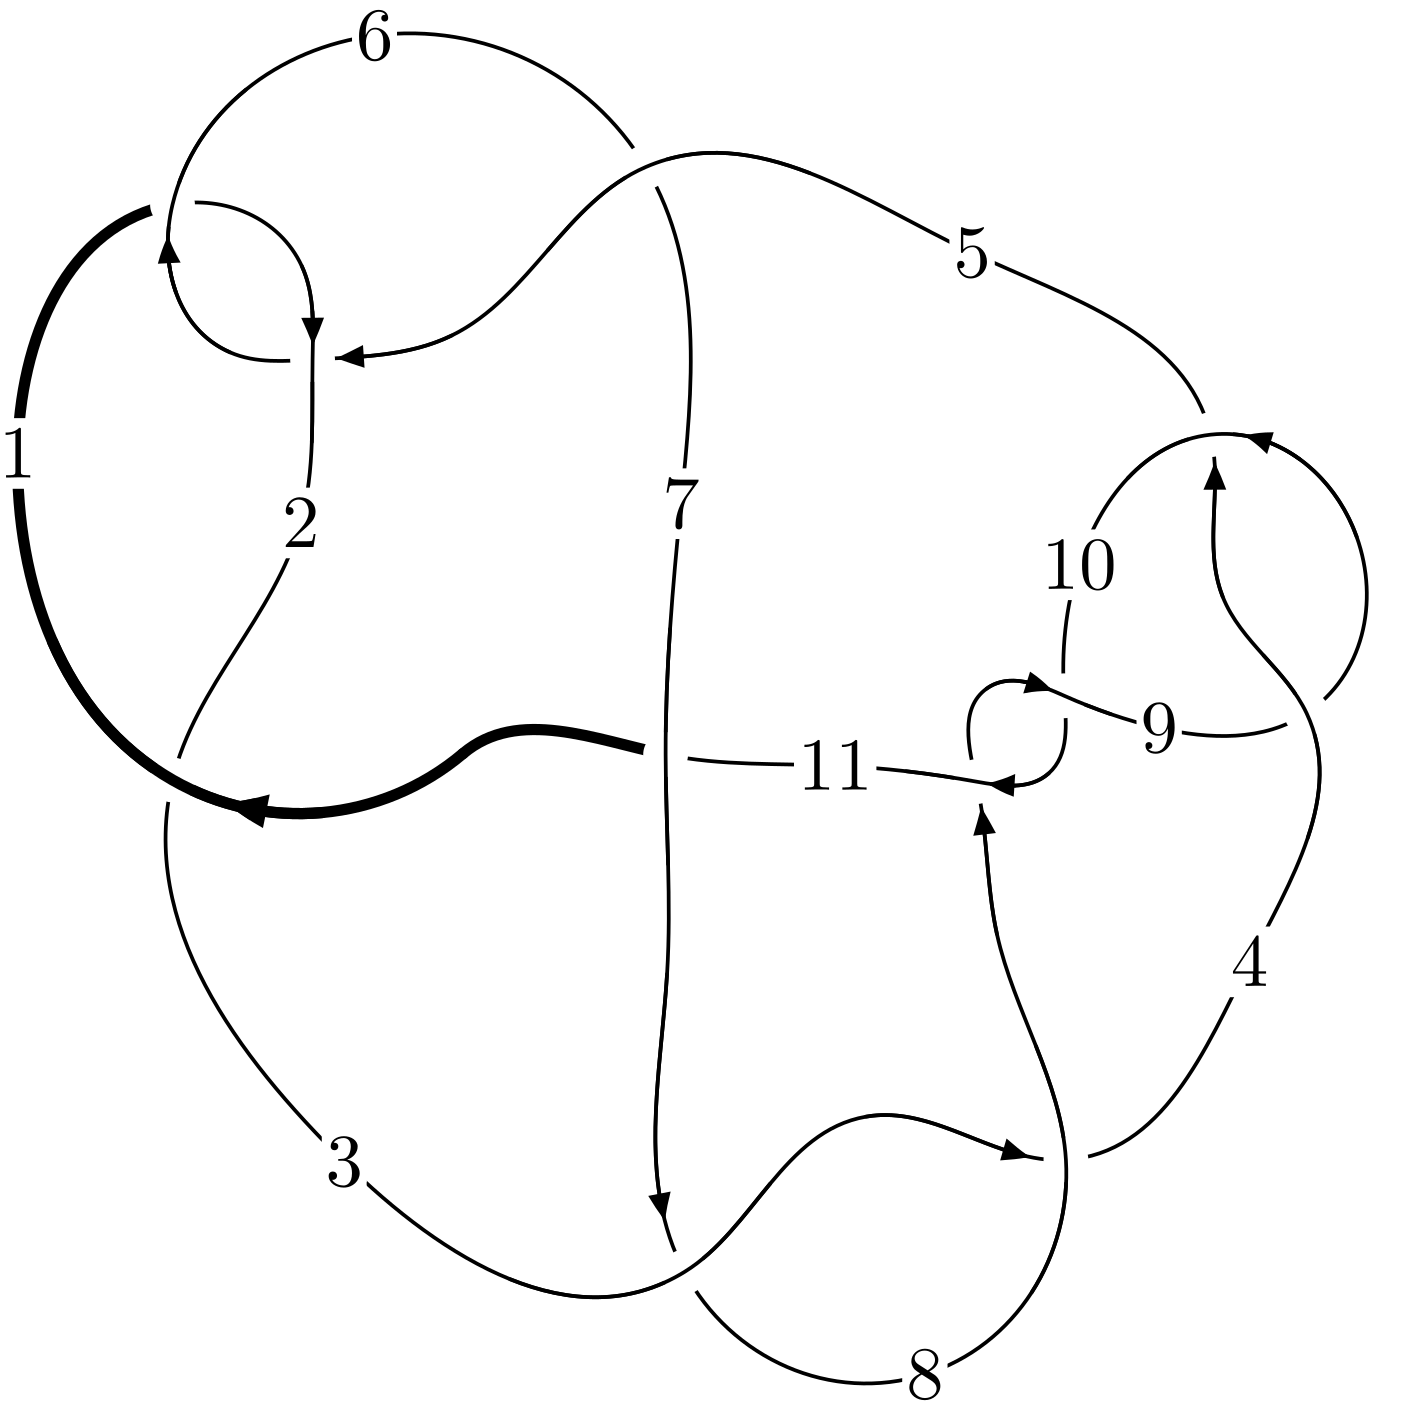
\includegraphics[width=112pt]{../../../GIT/diagram.site/Diagrams/png/369_11a_120.png}\\
\ \ \ A knot diagram\footnotemark}&
\allowdisplaybreaks
\textbf{Linearized knot diagam} \\
\cline{2-2}
 &
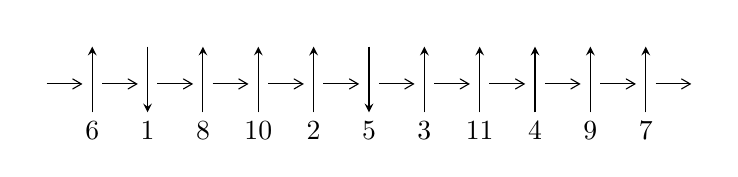
\begin{tikzpicture}[x=20pt, y=17pt]
	% nodes
	\node (C0) at (0, 0) {};
	\node (C1) at (1, 0) {};
	\node (C1U) at (1, +1) {};
	\node (C1D) at (1, -1) {6};

	\node (C2) at (2, 0) {};
	\node (C2U) at (2, +1) {};
	\node (C2D) at (2, -1) {1};

	\node (C3) at (3, 0) {};
	\node (C3U) at (3, +1) {};
	\node (C3D) at (3, -1) {8};

	\node (C4) at (4, 0) {};
	\node (C4U) at (4, +1) {};
	\node (C4D) at (4, -1) {10};

	\node (C5) at (5, 0) {};
	\node (C5U) at (5, +1) {};
	\node (C5D) at (5, -1) {2};

	\node (C6) at (6, 0) {};
	\node (C6U) at (6, +1) {};
	\node (C6D) at (6, -1) {5};

	\node (C7) at (7, 0) {};
	\node (C7U) at (7, +1) {};
	\node (C7D) at (7, -1) {3};

	\node (C8) at (8, 0) {};
	\node (C8U) at (8, +1) {};
	\node (C8D) at (8, -1) {11};

	\node (C9) at (9, 0) {};
	\node (C9U) at (9, +1) {};
	\node (C9D) at (9, -1) {4};

	\node (C10) at (10, 0) {};
	\node (C10U) at (10, +1) {};
	\node (C10D) at (10, -1) {9};

	\node (C11) at (11, 0) {};
	\node (C11U) at (11, +1) {};
	\node (C11D) at (11, -1) {7};
	\node (C12) at (12, 0) {};

	% arrows
	\draw[->,>={angle 60}]
	(C0) edge (C1) (C1) edge (C2) (C2) edge (C3) (C3) edge (C4) (C4) edge (C5) (C5) edge (C6) (C6) edge (C7) (C7) edge (C8) (C8) edge (C9) (C9) edge (C10) (C10) edge (C11) (C11) edge (C12) ;	\draw[->,>=stealth]
	(C1D) edge (C1U) (C2U) edge (C2D) (C3D) edge (C3U) (C4D) edge (C4U) (C5D) edge (C5U) (C6U) edge (C6D) (C7D) edge (C7U) (C8D) edge (C8U) (C9D) edge (C9U) (C10D) edge (C10U) (C11D) edge (C11U) ;
	\end{tikzpicture} \\
\hhline{~~} \\& 
\textbf{Solving Sequence} \\ \cline{2-2} 
 &
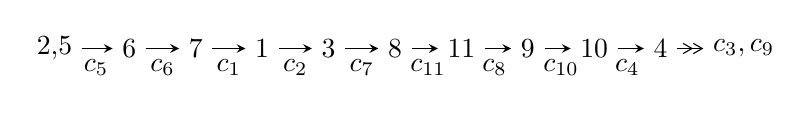
\begin{tikzpicture}[x=24pt, y=7pt]
	% node
	\node (A0) at (-1/8, 0) {2,5};
	\node (A1) at (1, 0) {6};
	\node (A2) at (2, 0) {7};
	\node (A3) at (3, 0) {1};
	\node (A4) at (4, 0) {3};
	\node (A5) at (5, 0) {8};
	\node (A6) at (6, 0) {11};
	\node (A7) at (7, 0) {9};
	\node (A8) at (8, 0) {10};
	\node (A9) at (9, 0) {4};
	\node (C1) at (1/2, -1) {$c_{5}$};
	\node (C2) at (3/2, -1) {$c_{6}$};
	\node (C3) at (5/2, -1) {$c_{1}$};
	\node (C4) at (7/2, -1) {$c_{2}$};
	\node (C5) at (9/2, -1) {$c_{7}$};
	\node (C6) at (11/2, -1) {$c_{11}$};
	\node (C7) at (13/2, -1) {$c_{8}$};
	\node (C8) at (15/2, -1) {$c_{10}$};
	\node (C9) at (17/2, -1) {$c_{4}$};
	\node (A10) at (41/4, 0) {$c_{3},c_{9}$};

	% edge
	\draw[->,>=stealth]	
	(A0) edge (A1) (A1) edge (A2) (A2) edge (A3) (A3) edge (A4) (A4) edge (A5) (A5) edge (A6) (A6) edge (A7) (A7) edge (A8) (A8) edge (A9) ;
	\draw[->>,>={angle 60}]	
	(A9) edge (A10);
\end{tikzpicture} \\ 

\end{tabular} \\

\footnotetext{
The image of knot diagram is generated by the software ``\textbf{Draw programme}" developed by Andrew Bartholomew(\url{http://www.layer8.co.uk/maths/draw/index.htm\#Running-draw}), where we modified some parts for our purpose(\url{https://github.com/CATsTAILs/LinksPainter}).
}\phantom \\ \newline 
\centering \textbf{Ideals for irreducible components\footnotemark of $X_{\text{par}}$} 
 
\begin{align*}
I^u_{1}&=\langle 
u^{54}- u^{53}+\cdots+3 u-1\rangle \\
\\
\end{align*}
\raggedright * 1 irreducible components of $\dim_{\mathbb{C}}=0$, with total 54 representations.\\
\footnotetext{All coefficients of polynomials are rational numbers. But the coefficients are sometimes approximated in decimal forms when there is not enough margin.}
\newpage
\renewcommand{\arraystretch}{1}
\centering \section*{I. $I^u_{1}= \langle u^{54}- u^{53}+\cdots+3 u-1 \rangle$}
\flushleft \textbf{(i) Arc colorings}\\
\begin{tabular}{m{7pt} m{180pt} m{7pt} m{180pt} }
\flushright $a_{2}=$&$\begin{pmatrix}0\\u\end{pmatrix}$ \\
\flushright $a_{5}=$&$\begin{pmatrix}1\\0\end{pmatrix}$ \\
\flushright $a_{6}=$&$\begin{pmatrix}1\\- u^2\end{pmatrix}$ \\
\flushright $a_{7}=$&$\begin{pmatrix}u^2+1\\- u^2\end{pmatrix}$ \\
\flushright $a_{1}=$&$\begin{pmatrix}- u\\u^3+u\end{pmatrix}$ \\
\flushright $a_{3}=$&$\begin{pmatrix}- u^3\\u^5+u^3+u\end{pmatrix}$ \\
\flushright $a_{8}=$&$\begin{pmatrix}u^{10}+u^8+2 u^6+u^4+u^2+1\\- u^{12}-2 u^{10}-4 u^8-4 u^6-3 u^4-2 u^2\end{pmatrix}$ \\
\flushright $a_{11}=$&$\begin{pmatrix}- u^7-2 u^5-2 u^3-2 u\\u^7+u^5+2 u^3+u\end{pmatrix}$ \\
\flushright $a_{9}=$&$\begin{pmatrix}- u^{26}-5 u^{24}+\cdots+3 u^2+1\\u^{26}+4 u^{24}+\cdots-4 u^4-3 u^2\end{pmatrix}$ \\
\flushright $a_{10}=$&$\begin{pmatrix}- u^{45}-8 u^{43}+\cdots-4 u^3-3 u\\u^{45}+7 u^{43}+\cdots+5 u^3+u\end{pmatrix}$ \\
\flushright $a_{4}=$&$\begin{pmatrix}u^{17}+2 u^{15}+5 u^{13}+6 u^{11}+7 u^9+6 u^7+4 u^5+2 u^3+u\\- u^{19}-3 u^{17}-8 u^{15}-13 u^{13}-17 u^{11}-17 u^9-12 u^7-6 u^5- u^3+u\end{pmatrix}$\\ \flushright $a_{4}=$&$\begin{pmatrix}u^{17}+2 u^{15}+5 u^{13}+6 u^{11}+7 u^9+6 u^7+4 u^5+2 u^3+u\\- u^{19}-3 u^{17}-8 u^{15}-13 u^{13}-17 u^{11}-17 u^9-12 u^7-6 u^5- u^3+u\end{pmatrix}$\\&\end{tabular}
\flushleft \textbf{(ii) Obstruction class $= -1$}\\~\\
\flushleft \textbf{(iii) Cusp Shapes $= 4 u^{53}+32 u^{51}+\cdots-8 u+14$}\\~\\
\newpage\renewcommand{\arraystretch}{1}
\flushleft \textbf{(iv) u-Polynomials at the component}\newline \\
\begin{tabular}{m{50pt}|m{274pt}}
Crossings & \hspace{64pt}u-Polynomials at each crossing \\
\hline $$\begin{aligned}c_{1},c_{5}\end{aligned}$$&$\begin{aligned}
&u^{54}- u^{53}+\cdots+3 u-1
\end{aligned}$\\
\hline $$\begin{aligned}c_{2},c_{6}\end{aligned}$$&$\begin{aligned}
&u^{54}+17 u^{53}+\cdots-5 u+1
\end{aligned}$\\
\hline $$\begin{aligned}c_{3},c_{7}\end{aligned}$$&$\begin{aligned}
&u^{54}- u^{53}+\cdots+5 u-25
\end{aligned}$\\
\hline $$\begin{aligned}c_{4},c_{9}\end{aligned}$$&$\begin{aligned}
&u^{54}+u^{53}+\cdots- u-1
\end{aligned}$\\
\hline $$\begin{aligned}c_{8},c_{10}\end{aligned}$$&$\begin{aligned}
&u^{54}-19 u^{53}+\cdots-5 u+1
\end{aligned}$\\
\hline $$\begin{aligned}c_{11}\end{aligned}$$&$\begin{aligned}
&u^{54}+5 u^{53}+\cdots-5 u-21
\end{aligned}$\\
\hline
\end{tabular}\\~\\
\newpage\renewcommand{\arraystretch}{1}
\flushleft \textbf{(v) Riley Polynomials at the component}\newline \\
\begin{tabular}{m{50pt}|m{274pt}}
Crossings & \hspace{64pt}Riley Polynomials at each crossing \\
\hline $$\begin{aligned}c_{1},c_{5}\end{aligned}$$&$\begin{aligned}
&y^{54}+17 y^{53}+\cdots-5 y+1
\end{aligned}$\\
\hline $$\begin{aligned}c_{2},c_{6}\end{aligned}$$&$\begin{aligned}
&y^{54}+41 y^{53}+\cdots-93 y+1
\end{aligned}$\\
\hline $$\begin{aligned}c_{3},c_{7}\end{aligned}$$&$\begin{aligned}
&y^{54}-39 y^{53}+\cdots-9225 y+625
\end{aligned}$\\
\hline $$\begin{aligned}c_{4},c_{9}\end{aligned}$$&$\begin{aligned}
&y^{54}-19 y^{53}+\cdots-5 y+1
\end{aligned}$\\
\hline $$\begin{aligned}c_{8},c_{10}\end{aligned}$$&$\begin{aligned}
&y^{54}+33 y^{53}+\cdots-13 y+1
\end{aligned}$\\
\hline $$\begin{aligned}c_{11}\end{aligned}$$&$\begin{aligned}
&y^{54}-11 y^{53}+\cdots+7283 y+441
\end{aligned}$\\
\hline
\end{tabular}\\~\\
\newpage\flushleft \textbf{(vi) Complex Volumes and Cusp Shapes}
$$\begin{array}{c|c|c}  
\text{Solutions to }I^u_{1}& \I (\text{vol} + \sqrt{-1}CS) & \text{Cusp shape}\\
 \hline 
\begin{aligned}
u &= -0.225158 + 0.985509 I\end{aligned}
 & \phantom{-}2.66174 - 2.82423 I & \phantom{-}9.41850 + 4.26927 I \\ \hline\begin{aligned}
u &= -0.225158 - 0.985509 I\end{aligned}
 & \phantom{-}2.66174 + 2.82423 I & \phantom{-}9.41850 - 4.26927 I \\ \hline\begin{aligned}
u &= \phantom{-}0.013188 + 1.020430 I\end{aligned}
 & -6.28584 + 2.76345 I & -1.40260 - 3.24602 I \\ \hline\begin{aligned}
u &= \phantom{-}0.013188 - 1.020430 I\end{aligned}
 & -6.28584 - 2.76345 I & -1.40260 + 3.24602 I \\ \hline\begin{aligned}
u &= -0.322299 + 0.910896 I\end{aligned}
 & -0.90934 + 3.04310 I & \phantom{-}5.53731 - 1.39630 I \\ \hline\begin{aligned}
u &= -0.322299 - 0.910896 I\end{aligned}
 & -0.90934 - 3.04310 I & \phantom{-}5.53731 + 1.39630 I \\ \hline\begin{aligned}
u &= \phantom{-}0.172024 + 1.019410 I\end{aligned}
 & -3.04751 + 3.37129 I & \phantom{-}1.74364 - 3.43225 I \\ \hline\begin{aligned}
u &= \phantom{-}0.172024 - 1.019410 I\end{aligned}
 & -3.04751 - 3.37129 I & \phantom{-}1.74364 + 3.43225 I \\ \hline\begin{aligned}
u &= -0.188352 + 1.032560 I\end{aligned}
 & -1.89570 - 8.85965 I & \phantom{-}3.95399 + 8.19419 I \\ \hline\begin{aligned}
u &= -0.188352 - 1.032560 I\end{aligned}
 & -1.89570 + 8.85965 I & \phantom{-}3.95399 - 8.19419 I \\ \hline\begin{aligned}
u &= \phantom{-}0.130465 + 0.911615 I\end{aligned}
 & -1.74890 + 1.55584 I & \phantom{-}1.72859 - 4.90109 I \\ \hline\begin{aligned}
u &= \phantom{-}0.130465 - 0.911615 I\end{aligned}
 & -1.74890 - 1.55584 I & \phantom{-}1.72859 + 4.90109 I \\ \hline\begin{aligned}
u &= -0.719799 + 0.809822 I\end{aligned}
 & \phantom{-}3.52747 - 0.23244 I & \phantom{-}13.19154 - 1.36658 I \\ \hline\begin{aligned}
u &= -0.719799 - 0.809822 I\end{aligned}
 & \phantom{-}3.52747 + 0.23244 I & \phantom{-}13.19154 + 1.36658 I \\ \hline\begin{aligned}
u &= -0.818638 + 0.718254 I\end{aligned}
 & \phantom{-}3.52513 + 2.90265 I & \phantom{-}8.89044 - 0.48035 I \\ \hline\begin{aligned}
u &= -0.818638 - 0.718254 I\end{aligned}
 & \phantom{-}3.52513 - 2.90265 I & \phantom{-}8.89044 + 0.48035 I \\ \hline\begin{aligned}
u &= \phantom{-}0.654895 + 0.871773 I\end{aligned}
 & \phantom{-}0.94675 + 2.54301 I & \phantom{-}4.57303 - 2.79240 I \\ \hline\begin{aligned}
u &= \phantom{-}0.654895 - 0.871773 I\end{aligned}
 & \phantom{-}0.94675 - 2.54301 I & \phantom{-}4.57303 + 2.79240 I \\ \hline\begin{aligned}
u &= \phantom{-}0.830157 + 0.717041 I\end{aligned}
 & \phantom{-}4.86571 - 8.43016 I & \phantom{-}10.90175 + 5.08103 I \\ \hline\begin{aligned}
u &= \phantom{-}0.830157 - 0.717041 I\end{aligned}
 & \phantom{-}4.86571 + 8.43016 I & \phantom{-}10.90175 - 5.08103 I \\ \hline\begin{aligned}
u &= -0.631705 + 0.643354 I\end{aligned}
 & -1.36873 + 3.22618 I & \phantom{-}6.44583 - 3.29326 I \\ \hline\begin{aligned}
u &= -0.631705 - 0.643354 I\end{aligned}
 & -1.36873 - 3.22618 I & \phantom{-}6.44583 + 3.29326 I \\ \hline\begin{aligned}
u &= -0.799923 + 0.758789 I\end{aligned}
 & \phantom{-}4.31402 + 0.26912 I & \phantom{-}9.66102 + 0. I\phantom{ +0.000000I} \\ \hline\begin{aligned}
u &= -0.799923 - 0.758789 I\end{aligned}
 & \phantom{-}4.31402 - 0.26912 I & \phantom{-}9.66102 + 0. I\phantom{ +0.000000I} \\ \hline\begin{aligned}
u &= \phantom{-}0.826542 + 0.743334 I\end{aligned}
 & \phantom{-}9.45805 - 1.89794 I & \phantom{-}15.5987 + 0. I\phantom{ +0.000000I} \\ \hline\begin{aligned}
u &= \phantom{-}0.826542 - 0.743334 I\end{aligned}
 & \phantom{-}9.45805 + 1.89794 I & \phantom{-}15.5987 + 0. I\phantom{ +0.000000I} \\ \hline\begin{aligned}
u &= \phantom{-}0.413630 + 0.782655 I\end{aligned}
 & -1.72347 + 2.04419 I & \phantom{-}4.15028 - 4.01557 I \\ \hline\begin{aligned}
u &= \phantom{-}0.413630 - 0.782655 I\end{aligned}
 & -1.72347 - 2.04419 I & \phantom{-}4.15028 + 4.01557 I \\ \hline\begin{aligned}
u &= \phantom{-}0.816023 + 0.773035 I\end{aligned}
 & \phantom{-}5.87973 + 4.75272 I & \phantom{-}12.23699 - 4.92141 I \\ \hline\begin{aligned}
u &= \phantom{-}0.816023 - 0.773035 I\end{aligned}
 & \phantom{-}5.87973 - 4.75272 I & \phantom{-}12.23699 + 4.92141 I\\
 \hline 
 \end{array}$$\newpage$$\begin{array}{c|c|c}  
\text{Solutions to }I^u_{1}& \I (\text{vol} + \sqrt{-1}CS) & \text{Cusp shape}\\
 \hline 
\begin{aligned}
u &= \phantom{-}0.637029 + 0.965427 I\end{aligned}
 & -2.61478 + 2.76089 I & \phantom{-}3.34853 + 0. I\phantom{ +0.000000I} \\ \hline\begin{aligned}
u &= \phantom{-}0.637029 - 0.965427 I\end{aligned}
 & -2.61478 - 2.76089 I & \phantom{-}3.34853 + 0. I\phantom{ +0.000000I} \\ \hline\begin{aligned}
u &= -0.713272 + 0.912768 I\end{aligned}
 & \phantom{-}3.21684 - 5.24753 I & \phantom{-}12.07775 + 7.28540 I \\ \hline\begin{aligned}
u &= -0.713272 - 0.912768 I\end{aligned}
 & \phantom{-}3.21684 + 5.24753 I & \phantom{-}12.07775 - 7.28540 I \\ \hline\begin{aligned}
u &= -0.652949 + 0.976409 I\end{aligned}
 & -2.30035 - 8.30381 I & \phantom{-0.000000 -}0. + 8.62112 I \\ \hline\begin{aligned}
u &= -0.652949 - 0.976409 I\end{aligned}
 & -2.30035 + 8.30381 I & \phantom{-0.000000 } 0. - 8.62112 I \\ \hline\begin{aligned}
u &= \phantom{-}0.501769 + 0.617981 I\end{aligned}
 & -1.73704 + 2.07051 I & \phantom{-}5.30183 - 3.63568 I \\ \hline\begin{aligned}
u &= \phantom{-}0.501769 - 0.617981 I\end{aligned}
 & -1.73704 - 2.07051 I & \phantom{-}5.30183 + 3.63568 I \\ \hline\begin{aligned}
u &= -0.738963 + 0.973368 I\end{aligned}
 & \phantom{-}3.65451 - 6.06207 I & \phantom{-0.000000 } 0 \\ \hline\begin{aligned}
u &= -0.738963 - 0.973368 I\end{aligned}
 & \phantom{-}3.65451 + 6.06207 I & \phantom{-0.000000 } 0 \\ \hline\begin{aligned}
u &= \phantom{-}0.755217 + 0.969347 I\end{aligned}
 & \phantom{-}5.27505 + 1.13830 I & \phantom{-0.000000 } 0 \\ \hline\begin{aligned}
u &= \phantom{-}0.755217 - 0.969347 I\end{aligned}
 & \phantom{-}5.27505 - 1.13830 I & \phantom{-0.000000 } 0 \\ \hline\begin{aligned}
u &= \phantom{-}0.749443 + 0.991696 I\end{aligned}
 & \phantom{-}8.69493 + 7.80028 I & \phantom{-0.000000 } 0 \\ \hline\begin{aligned}
u &= \phantom{-}0.749443 - 0.991696 I\end{aligned}
 & \phantom{-}8.69493 - 7.80028 I & \phantom{-0.000000 } 0 \\ \hline\begin{aligned}
u &= -0.735797 + 1.001920 I\end{aligned}
 & \phantom{-}2.65813 - 8.73650 I & \phantom{-0.000000 } 0 \\ \hline\begin{aligned}
u &= -0.735797 - 1.001920 I\end{aligned}
 & \phantom{-}2.65813 + 8.73650 I & \phantom{-0.000000 } 0 \\ \hline\begin{aligned}
u &= \phantom{-}0.740821 + 1.006800 I\end{aligned}
 & \phantom{-}3.9780 + 14.3126 I & \phantom{-0.000000 } 0 \\ \hline\begin{aligned}
u &= \phantom{-}0.740821 - 1.006800 I\end{aligned}
 & \phantom{-}3.9780 - 14.3126 I & \phantom{-0.000000 } 0 \\ \hline\begin{aligned}
u &= -0.638480 + 0.083682 I\end{aligned}
 & \phantom{-}1.68643 - 6.22008 I & \phantom{-}11.41350 + 5.62288 I \\ \hline\begin{aligned}
u &= -0.638480 - 0.083682 I\end{aligned}
 & \phantom{-}1.68643 + 6.22008 I & \phantom{-}11.41350 - 5.62288 I \\ \hline\begin{aligned}
u &= -0.633762\phantom{ +0.000000I}\end{aligned}
 & \phantom{-}5.79098\phantom{ +0.000000I} & \phantom{-}16.1980\phantom{ +0.000000I} \\ \hline\begin{aligned}
u &= \phantom{-}0.593562 + 0.088163 I\end{aligned}
 & \phantom{-}0.459602 + 0.933389 I & \phantom{-}9.53888 - 0.84977 I \\ \hline\begin{aligned}
u &= \phantom{-}0.593562 - 0.088163 I\end{aligned}
 & \phantom{-}0.459602 - 0.933389 I & \phantom{-}9.53888 + 0.84977 I \\ \hline\begin{aligned}
u &= \phantom{-}0.334907\phantom{ +0.000000I}\end{aligned}
 & \phantom{-}0.694593\phantom{ +0.000000I} & \phantom{-}14.5890\phantom{ +0.000000I}\\
 \hline 
 \end{array}$$\newpage
\newpage\renewcommand{\arraystretch}{1}
\centering \section*{ II. u-Polynomials}
\begin{tabular}{m{50pt}|m{274pt}}
Crossings & \hspace{64pt}u-Polynomials at each crossing \\
\hline $$\begin{aligned}c_{1},c_{5}\end{aligned}$$&$\begin{aligned}
&u^{54}- u^{53}+\cdots+3 u-1
\end{aligned}$\\
\hline $$\begin{aligned}c_{2},c_{6}\end{aligned}$$&$\begin{aligned}
&u^{54}+17 u^{53}+\cdots-5 u+1
\end{aligned}$\\
\hline $$\begin{aligned}c_{3},c_{7}\end{aligned}$$&$\begin{aligned}
&u^{54}- u^{53}+\cdots+5 u-25
\end{aligned}$\\
\hline $$\begin{aligned}c_{4},c_{9}\end{aligned}$$&$\begin{aligned}
&u^{54}+u^{53}+\cdots- u-1
\end{aligned}$\\
\hline $$\begin{aligned}c_{8},c_{10}\end{aligned}$$&$\begin{aligned}
&u^{54}-19 u^{53}+\cdots-5 u+1
\end{aligned}$\\
\hline $$\begin{aligned}c_{11}\end{aligned}$$&$\begin{aligned}
&u^{54}+5 u^{53}+\cdots-5 u-21
\end{aligned}$\\
\hline
\end{tabular}\newpage\renewcommand{\arraystretch}{1}
\centering \section*{ III. Riley Polynomials}
\begin{tabular}{m{50pt}|m{274pt}}
Crossings & \hspace{64pt}Riley Polynomials at each crossing \\
\hline $$\begin{aligned}c_{1},c_{5}\end{aligned}$$&$\begin{aligned}
&y^{54}+17 y^{53}+\cdots-5 y+1
\end{aligned}$\\
\hline $$\begin{aligned}c_{2},c_{6}\end{aligned}$$&$\begin{aligned}
&y^{54}+41 y^{53}+\cdots-93 y+1
\end{aligned}$\\
\hline $$\begin{aligned}c_{3},c_{7}\end{aligned}$$&$\begin{aligned}
&y^{54}-39 y^{53}+\cdots-9225 y+625
\end{aligned}$\\
\hline $$\begin{aligned}c_{4},c_{9}\end{aligned}$$&$\begin{aligned}
&y^{54}-19 y^{53}+\cdots-5 y+1
\end{aligned}$\\
\hline $$\begin{aligned}c_{8},c_{10}\end{aligned}$$&$\begin{aligned}
&y^{54}+33 y^{53}+\cdots-13 y+1
\end{aligned}$\\
\hline $$\begin{aligned}c_{11}\end{aligned}$$&$\begin{aligned}
&y^{54}-11 y^{53}+\cdots+7283 y+441
\end{aligned}$\\
\hline
\end{tabular}
\vskip 2pc
\end{document}